\newpage
\section{Results}
% General structure.
% Display spectrums, try to calculate quality factor at least.
% Display some prelimary purities.
% Some stuff I probably should have calculated:
% Powers in the waveguide, peak power
\subsection{Glassgow}
This chip was used to do an initial proof of concept that the JSI of a ring resonator could be measured at high resolution. Here the aim was to explore different ring geometries and develop an intuition on how to do the experiment. The Pritel pulsed laser was used with a pulse duration of \SI{2}{\pico\second}, a FWHM of \SI{1.0}{\nano\meter} with wavelength range \SI{1530}{\nano\meter} to \SI{1530}{\nano\meter} and a peak power of \SI{100}{\watt}. Due to the pulsed laser sometimes destroying the spot size converter on the chip a \SI{3}{\decibel} attenuator was added just after the laser output, this resulted in roughly about \SI{5}{\deci\bel\m} of power coming out of the lense fiber.

As each device on the chip has unique characteristics due to fabrication errors only some devices produced good data meaning that a full characterisation of the chip was not possible and only a few devices were used. Typically it was imperfections in the spot size converters on the chips being imperfect which prevented good JSI's from being collected but another issue encountered was under coupling of the rings.

Here we present three data sets collected, each has high SNR of at least $20$ allowing for the maximum purity $P_{max}$ to be calculated with high accuracy. The relevant spectral scan is presented with the JSIs for reference, these are routine scans performed with the tunable CW laser typically at \SI{1}{\m\watt} of which roughly \SI{-14}{\deci\bel\m} gets into the chip. 

% RING C17
\begingroup
    \centering  
    \includegraphics[width=15cm]{/home/luka/Dropbox/cqp/report/thesis/res/glassgow/C17/graph.pdf}
    \captionof{figure}{{\bf JSI Ring C17} We calculate a quality factor of $Q \approx 25000$. In this instance the coupling loss was on average \SI{20}{\dB} and the input power of the pulsed laser was \SI{5.1}{\dB} giving a estimated power in waveguide of \SI{-5}{\dB}. The probe laser operated at \SI{1}{\m\watt}. Fitting the spectral scans of the ring resonators gives coupling parameters of the order $r=0.946$ $\tau = 0.985$ $n_{eff} = 4.136$, note these are only estimates.} 
     \vspace{3pt} \label{c17_jsi}
\endgroup

% C17 key points
% it works, SW stuff interferes and is of lower intensity, it happens before the ring


Figure \ref{c17_jsi} shows a clear response from the ring resonator at the resonant frequencies, superimposed on this there is also straight waveguide stimulated four wave mixing observed at much lower intensities. It can be deduced that much of this straight wave guide contribution happens before the ring as it is filtered at the resonance wavelength.
The asymmetry is an experimental artefact of imperfect alignment of the resonances with the AWG channels and the pump laser. This is  $P_{max}$ value.

% RING C21
\begingroup
    \centering  
    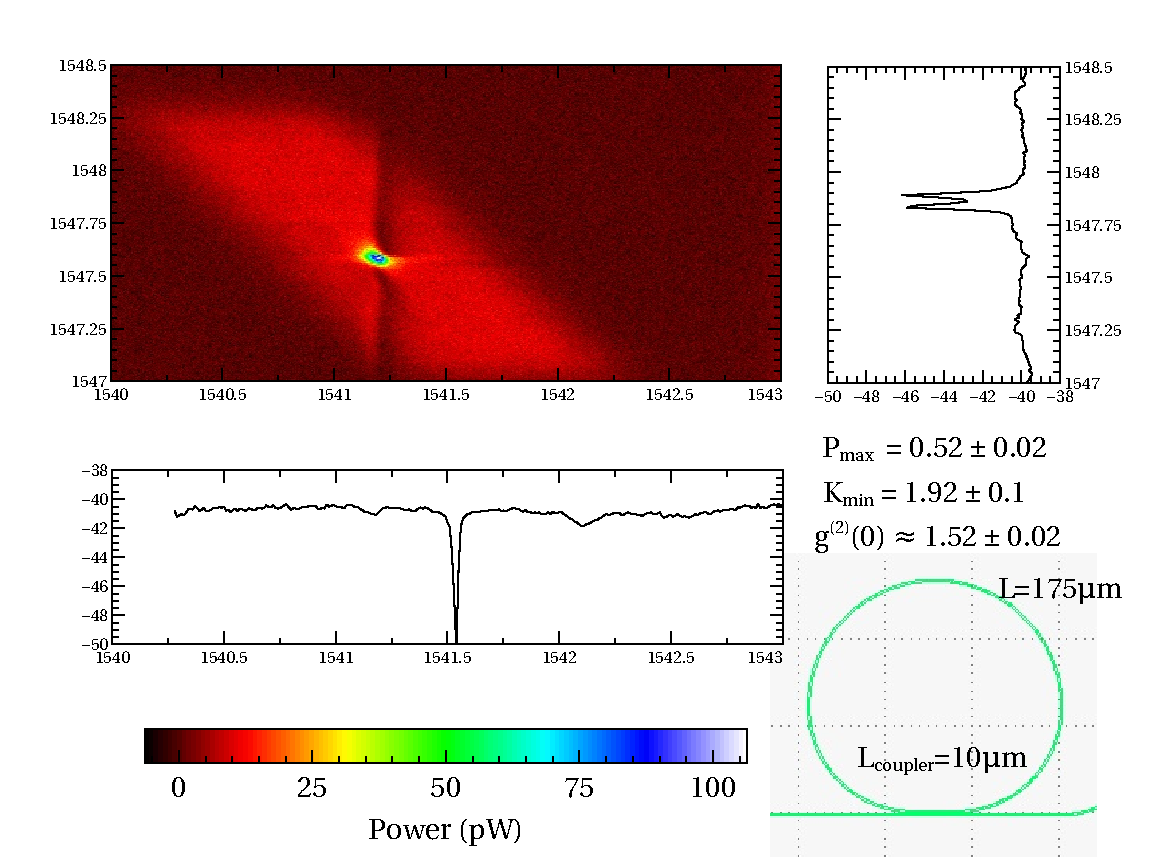
\includegraphics[width=15cm]{/home/luka/Dropbox/cqp/report/thesis/res/glassgow/C21/c21graph.pdf}
    \captionof{figure}{{\bf JSI Ring C21} We calculate a quality factor of $Q \approx 28000$. In this instance the coupling loss was on average \SI{21}{\dB} and the input power of the pulsed laser was \SI{5.5}{\deci\bel\m} giving a estimated power in waveguide of \SI{-5}{\deci\bel\m}. The probe laser operated at \SI{1}{\m\watt}. Fitting the spectral scans of the ring resonators gives coupling parameters of the order $r=0.957$ $\tau = 0.977$ $n_{eff} = 4.144$, note these are only estimates.} 
     \vspace{3pt} \label{c21_jsi}
\endgroup

In figure \ref{c21_jsi} we see ring C21 which has has many physical similarities with ring C17 shown in figure \ref{c17_jsi} however we observe a few key differences. Firstly the resonance that the CW laser probes is split but this is not reflected in the JSI because the split feature is on the order of \SI{0.01}{\nano\meter} which under the \SI{0.03}{\nano\meter} resolution of the OSA. This inability to resolve finer features which are almost certainly encoded in the real JSA is an important topic discussed later on in this work.

Secondly the coupling distance of the egg shaped resonator is slightly shorter here which is reflected in a slightly smaller value for $r$, however this difference isn't significant enough to use for a comparison as there are many other factors between the two experiments that were not held constant, in particular the alignment of the AWG channels.

% RING B32
\begingroup
    \centering  
    \includegraphics[width=15cm]{/home/luka/Dropbox/cqp/report/thesis/res/glassgow/B32/graph.pdf}
    \captionof{figure}{{\bf JSI Ring B32} We calculate a quality factor of $Q \approx 14000$. In this instance the coupling loss was on average \SI{22}{\deci\bel\m} and the input power of the pulsed laser was \SI{5.1}{\deci\bel\m} giving a estimated power in waveguide of \SI{0}{\deci\bel\m}. The probe laser operated at \SI{1}{\m\watt}. Fitting the spectral scans of the ring resonators gives coupling parameters of the order $r=0.985$ $\tau = 0.947$ $n_{eff} = 4.136$, note these are only estimates. } 
     \vspace{3pt} \label{b32_jsi}
\endgroup

The final JSI collected for this chip is shown in figure \ref{b32_jsi}, here the ring geometry is of the more traditional circular shape. It is observed that the resonance has some asymmetry due to more prominent non-linear effects. We observe the intensities of the ring resonator and straight wave guide FWM processes to be more similar in this scan which can be accounted for by the lower quality factory. Again it is notable to see that the ring seems to be collecting some of the straight wave guide FWM, however at a shifted frequency to the peak of the ring FWM, this is contradictory to the two previous examples and may be due to the more non-linear response of this ring.
\newline\newline
\noindent
{\bf Summary }The three purities observed $(0.42,0.52,0.62)$ coincide with previous characterisations of the chip using the single photon detectors which measured a purity of on the order 0.45 \cite{scammell_indistinguishable_2014}. A advantage to these measurements is they allow one to easier develop ways of increasing the purity.
\subsection{a-Si}

% Some initial joint spectrums.
% Try to calculate the quality of the rings.
% Analyse the g2(0) data

% asi
\begingroup
    \centering  
    \includegraphics[width=16cm]{/home/luka/Dropbox/cqp/report/thesis/res/asi/graph.pdf}
    \captionof{figure}{{\bf JSI Ring C21} We calculate a quality factor of $Q \approx 28000$. In this instance the coupling loss was on average \SI{21}{\dB} and the input power of the pulsed laser was \SI{5.5}{\deci\bel\m} giving a estimated power in waveguide of \SI{-5}{\deci\bel\m}. The probe laser operated at \SI{1}{\m\watt}. Fitting the spectral scans of the ring resonators gives coupling parameters of the order $r=0.957$ $\tau = 0.977$ $n_{eff} = 4.144$, note these are only estimates.} 
     \vspace{3pt} \label{asi_jsi_grid}
\endgroup

\subsection{Toshiba}

\subsubsection{Bistability Data}
% Should be easy
\subsubsection{Pulse shaping}
% Touch on the pulse shaping experiment
\subsubsection{Power Scans}
%